\chapter{Meta-Feature Guided Regularized Regression for Survival Outcomes}
\label{cha:xtunecox}

\section{Abstract}
Regularized regression is a widely used technique for building prognostic and diagnostic models based on genomic features. Regularized regression can handle high-dimensional data common in genomic studies, and in the case of sparse regularized methods  it can also  perform feature selection. Associated with genomic features, such as gene expression, genotypes and DNA methylation, there is a great deal of functional information that, if directly incorporated into the modeling process, could yield better prediction performance. Examples of functional information are pathways and other gene sets, gene ontology annotations, and knowledge from previous studies. Functional information can often be represented as meta-features, i.e. attributes of the features rather than of the subjects. 

In this chapter, we extend the approach of \cite{zeng2021incorporating} to survival outcomes. The method can incorporate prior information in the form of meta-features to guide regularized Cox regression models. This is accomplished by letting each genomic feature to have its own `custom' penalty parameter, rather than having a single penalty parameter controlling the degree of regularization across all features. The individual penalty parameters are in turn modeled to be functions of the meta-features.  We show the benefits of the method by a simulation study and applications to two genomic studies.  

\section{Introduction}
Predicting health outcomes based on genomic profiles is an important and active area of Biomedical research. A commonly used statistical tool for developing predictive model in genomic studies is regularized regression. When the number of features is larger than the number of samples, which is usually the case for genomic data, regularization needs to be introduced so that the model complexity, relative to the amount of data available, can be controlled. Sparse regularized regression is a popular choice, as it not only shrinks the regression coefficients toward zero to make the model less complex by reducing its variance, but it also shrinks some of the coefficients with small or no effect on the outcome to exactly zero, thereby performing feature selection. The most widely used  sparse regularized regression methods are the lasso \citep{tibshirani1996regression} and the elastic net \citep{zou2005regularization}. While the lasso and elastic net share many properties, the elastic net can better deal with correlated features. Specifically,  while the lasso tends to select a single feature among a highly correlated group of features predictive of the outcome, the elastic net tends to select the entire group and make their effect-size estimates similar to each other. Ridge regression \citep{hoerl1970ridge} is another widely used regularization technique to cope with high-dimensional and collinear data. However, ridge regression does not yield sparse models, i.e. it does not perform feature selection. 

Several extensions of the lasso have been developed to exploit additional structure of the features such as groupings or natural orderings. For example, the group lasso \citep{yuan2006model} takes grouping information such as genes mapping to a pathway or probes mapping to a a gene, and shrinks the coefficients by group so that either all the features in a group are selected or no feature in the group is selected. The sparse group lasso \citep{simon2013sparse} further allows sparsity within each group. The fused lasso deals with the setting where an ordering of the features is available (e.g. along the genome), by adding an $L_1$ penalty for the differences of neighbouring coefficients. The above extend regularized  regression methods to account for attributes of the features, which can be often encoded as features of the features or meta-features. Example of meta-features common in genomic studies are functional gene sets like hallmark \citep{liberzon2015molecular}, gene ontology pathways like those in the Reactome database \citep{jassal2020reactome}, and summary statistics like p-values and regression coefficients from meta-analyses or other previous relevant work. Meta-features can be encoded as data matrices, where the samples/rows represent the features, and the columns represent the meta-features. None of the regularization approaches above can systematically utilize general meta-feature information. For example, the group lasso requires features in different groups to be mutually exclusive. The fused lasso can incorporate an ordering of the features into account, which can be captured by a single quantitative meta-feature, but it is not designed to integrate multiple quantitative meta-features. 

One way of utilizing functional meta-features that define groupings is by performing gene set enrichment analysis \citep{subramanian2005gene} after identifying features that are predictive of the outcome of interest. However, incorporating meta-features directly into the modeling process can potentially improve both prediction performance and the quality of feature selection. In chapter \ref{cha:xrnetcox}, we incorporated  meta-features in a hierarchical fashion, in an approach that can be conceptualized as regressing the outcome on the original features, 
$ \bm{Y} = \bm{X\beta} + \bm{\varepsilon} $, 
where $\bm{Y}$ is the length $n$ outcome vector, $\bm{X}$ is the $n \times p$ data matrix, $\bm{\beta}$ is the length $p$ feature coefficient vector to be estimated in the model, and then regressing the estimates $\bm{\beta}$ on the meta-features, $\bm{\beta} = \bm{Z\alpha} + \bm{\gamma}$, where $\bm{Z}$ is the $p \times q$ meta-feature matrix, $\bm{\alpha}$ is coefficients vector for meta-features. To integrate both features and meta features jointly, an optimization problem is formulated as follows: 
$$ \min_{\bm{\beta, \alpha}} \frac{1}{2n} \|\bm{Y}-\bm{X \beta} \|_2^2 + \frac{\lambda_1}{2} \|\bm{\beta} - \bm{Z \alpha} \|_2^2 + \lambda_2 \|\bm{\alpha}\|_1 $$
The feature data, $\bm{X}$, and the meta-feature data, $\bm{Z}$, are both integrated  through the $L_2$ terms. The additional $L_1$ term penalizes the meta-feature coefficients $\bm{\alpha}$ to control the model complexity and perform meta-feature selection. This approach incorporates meta-features in a linear way. In Chapter 2 it was shown that this approach can considerably improve the prediction performance of regularized Cox regression  when integrating informative meta-features. \cite{zeng2021incorporating} developed an alternative method for integrating meta-features $\bm{Z}$ in a non-linear way, for quantitative and binary outcomes. This is accomplished by letting each feature have its own `customized' penalty parameter, rather than a single global penalty parameter for all features. The customized penalty parameter approach can also improve prediction performance and feature selection. In this chapter, we extend this approach to survival outcomes. 

\section{Methods}
\subsection{Setup and notation}
Starting with the time-to-event model setup, we let the outcome be $(\bm{y, \delta})$ where $\bm{y}=(y_1,y_2,\dots,y_n)$ denotes the vector of observed times, and $\bm{\delta}=(\delta_1,\delta_2,\dots,\delta_n)$ denotes the vector of censoring status for the $n$ subjects. For subject $i$, $i=1,2,\dots,n$, $\delta_i = 1$  if the event of interest (e.g., death) took place within the followup period and $y_i$ is time of the event; if $\delta_i=0$, the event did not happen within the followup period, and $y_i$ is the censoring time. We assume there are $p$ genomic features (e.g. expression or methylation levels, genotypes), measured on each of the $n$ subjects. The  $n\times p$ data matrix $\bm{X}$ stores the feature values, i.e., $\bm{x}_i = (x_{i1},x_{i2},\dots,x_{ip})$ is a vector of feature values for subject $i$. Associated with the features, we assume there are $q$ meta-features. A $p\times q$ matrix $\bm{Z}$ stores the meta-feature values for the $p$ original features, i.e., $\bm{z}_j = (z_{j1},z_{j2},\dots,z_{jq})$ for  $j=1,2,\dots,p$ is a vector of meta-feature values for feature $j$. The most common  regression method for time-to-event data is Cox's proportional hazards model \citep{cox1972regression}. It assumes proportional hazard functions with respect to feature values at the same time point, which allows model fitting without explicitly knowing the form of the baseline hazard function, and  depending only on the order in which events occur, but not on the exact time of occurrence. We let $t_1 \le t_2 \le \dots \le t_l \le \dots \le  t_m$ be the event times arranged in increasing order and $D_l=\{i:\delta_i=1,y_i=t_l\}$ be the set of subjects that experienced the event at time $t_l$. Letting $\bm{\beta}$ be a length $p$ vector of regression coefficients, Breslow's adjustment to the Cox partial likelihood \citep{breslow1972contribution} takes the form: 
\begin{displaymath}
L(\bm{\beta}) = \prod_{l=1}^{m} \frac{e^{\sum_{i\in D_l}\bm{x}_i^T\bm{\beta}}}{(\sum_{i\in R_l} e^{\bm{x}_i^T\bm{\beta}})^{d_l}}
\end{displaymath}
where $R_l=\{i: y_i\geq t_l\}$ is the risk set at event time $t_l$, i.e., the set of all subjects who have not experienced the event and are uncensored just prior to time $t_l$, and $d_l=|D_l|$ is the number of events at time $t_l$.  Breslow's partial likelihood handles potential ties at each event time (i.e., more than one subject experiencing the event at the same time). When there are no ties, $L(\bm{\beta})$ automatically reduces to Cox's partial likelihood. We can see that neither the hazard functions nor the actual times are involved in the partial likelihood, only the order of event times matters. 

To control the model complexity we consider an elastic net regularized Cox model. Denoting the log partial likelihood by $\ell(\bm{\beta})$, the regularized Cox regression model is the solution to the following optimization problem:
\begin{equation} \label{eq1}
    \min_{\bm{\beta}\in \mathbb{R}^p} \left\{-\ell(\bm{\beta}) + \lambda\left[\frac{1}{2}(1-c)\|\bm{\beta}\|_2^2 + c\|\bm{\beta}\|_1\right]\right\}.
\end{equation}
The regularization function includes the lasso ($c=1$), elastic net ($0 < c <1)$, and ridge ($c=0$) penalties as particular cases. When $ 0<c \leq 1$, the penalty is sparse inducing, i.e.,  shrink some coefficients to exactly zero, producing more interpretable models. In \eqref{eq1} the global penalty parameter $\lambda$ is the same  for all the features, which implicitly assumes all features are a priori equally important.  To incorporate meta-features which might be informative about the importance of the features, we give each feature its own unique penalty parameter $\lambda_j$, which in turn we model to be a function of the meta-features. Specifically,  we assume $\lambda_j=e^{\bm{z_j}^T \bm{\alpha}}$ where $\bm{\alpha}$ is a weight vector of length $q$. The model is now given by the following optimization problem: 
\begin{equation} \label{eq2}
\begin{aligned}
    &\min_{\bm{\beta}\in \mathbb{R}^p} \left\{-\ell(\bm{\beta}) + \sum_{j=1}^p \lambda_j\left[\frac{1}{2}(1-c)\beta_j^2 + c|\beta_j|\right]\right\}, \\
    &\lambda_j = e^{\bm{z_j}^T \bm{\alpha}}.
\end{aligned}
\end{equation}

\subsection{Model fitting}
The standard elastic net Cox proportional hazards model in equation \eqref{eq1}, can be fitted by pathwise coordinate descent \citep{simon2011regularization}. Since the  penalty parameter $\lambda$ is a global hyper-parameter, the algorithm typically constructs a grid of $\lambda$ values from which the best is selected by cross-validation. By contrast, the proposed model in equation \eqref{eq2}, has $p$ $\lambda$'s defined by the weights as $\bm{\alpha}$, $\bm{\lambda} = (\lambda_1,\lambda_2,\dots,\lambda_p) = e^{\bm{Z\alpha}}$, so it is not feasible to tune them using traditional approaches like cross-validation. Instead, we estimate the weights $\bm{\alpha}$ to get the  $\bm{\lambda}$ directly based on the data using an empirical-Bayes approach. With known $\bm{\lambda}$, the model in \eqref{eq2} can be fit via coordinate descent.

\subsubsection{Empirical Bayes estimation of the hyperparameters} \label{laplace}
To estimate $\bm{\alpha}$, we rely on an alternative and natural Bayesian/random effects formulation of the model in \eqref{eq2}. We then estimate the hyper-parameters by maximizing the marginal likelihood obtained by integrating out the random effects $\bm{\beta}$. Based on the Bayesian elastic net \citep{li2010bayesian}, the model given by equation \eqref{eq2} can be re-formulated as the following hierarchical model:
\begin{align}
    &f(\bm{Y}|\bm{\beta}; \bm{X}) = \prod_{l=1}^{m} \frac{e^{\sum_{i\in D_l}\bm{x}_i^T\bm{\beta}}}{(\sum_{i\in R_l} e^{\bm{x}_i^T\bm{\beta}})^{d_l}} \label{eq3}, \\
    &\pi(\beta_j; \bm{\alpha}) \propto exp\left\{ -\lambda_j\left[\frac{1}{2}(1-c)\beta_j^2 + c|\beta_j|\right] \right\}. \label{eq4}
\end{align}
With the likelihood \eqref{eq3} and prior distribution \eqref{eq4}, we construct the joint distribution of $\bm{Y}$ and $\bm{\beta}$, and integrate out $\bm{\beta}$, so to get the marginal likelihood of $\bm{Y}$:
\begin{align*}
f(\bm{Y};\bm{\alpha}) &= \int_{\bm{\beta}\in\mathbb{R}^p} f(\bm{Y}, \bm{\beta};\bm{\alpha}) d\bm{\beta} \\
&= \int_{\bm{\beta}\in\mathbb{R}^p} f(\bm{Y}|\bm{\beta};\bm{X}) \pi(\bm{\beta};\bm{\alpha})d\bm{\beta} \\
&= \int_{\bm{\beta}\in\mathbb{R}^p} \prod_{l=1}^{m} \frac{e^{\sum_{i\in D_l}\bm{x}_i^T\bm{\beta}}}{(\sum_{i\in R_l} e^{\bm{x}_i^T\bm{\beta}})^{d_l}} \prod_{j=1}^{p}exp\left\{ -\lambda_j\left[\frac{1}{2}(1-c)\beta_j^2 + c|\beta_j|\right] \right\}  d\bm{\beta}
\end{align*} 
This integral does not have a closed form expression because the elastic net prior is not conjugate for the likelihood. We propose to approximate the integral by first approximating the elastic net prior with a normal prior, and then  applying the Laplace approximation to get a tractable final approximation. To approximate the elastic net prior, we use a normal prior with the same variance as the lasso component. The lasso component of the prior corresponds to a double exponential distribution, $DE(\lambda_jc)$, with variance $\frac{2}{(\lambda_jc)^2}$. The normal approximation of this double exponential distribution is then $N(0, \frac{2}{(\lambda_jc)^2})$. Hence, the elastic net prior can be approximated as follow,
\begin{equation} \label{eq5}
\begin{aligned}
    \pi(\beta_j; \bm{\alpha}) &\propto exp\left\{ -\lambda_j\left[\frac{1}{2}(1-c)\beta_j^2 + c|\beta_j|\right] \right\} \\
    &\approx exp\left\{ -\frac{1}{2}\lambda_j(1-c)\beta_j^2 + \frac{\beta_j^2}{2(\frac{2}{(\lambda_jc})^2} \right\} \\
    &= N \left( 0, \frac{2}{2\lambda_j(1-c)+c^2\lambda_j^2} \right). 
\end{aligned}
\end{equation}
\begin{figure}[tbh]
  \centering
  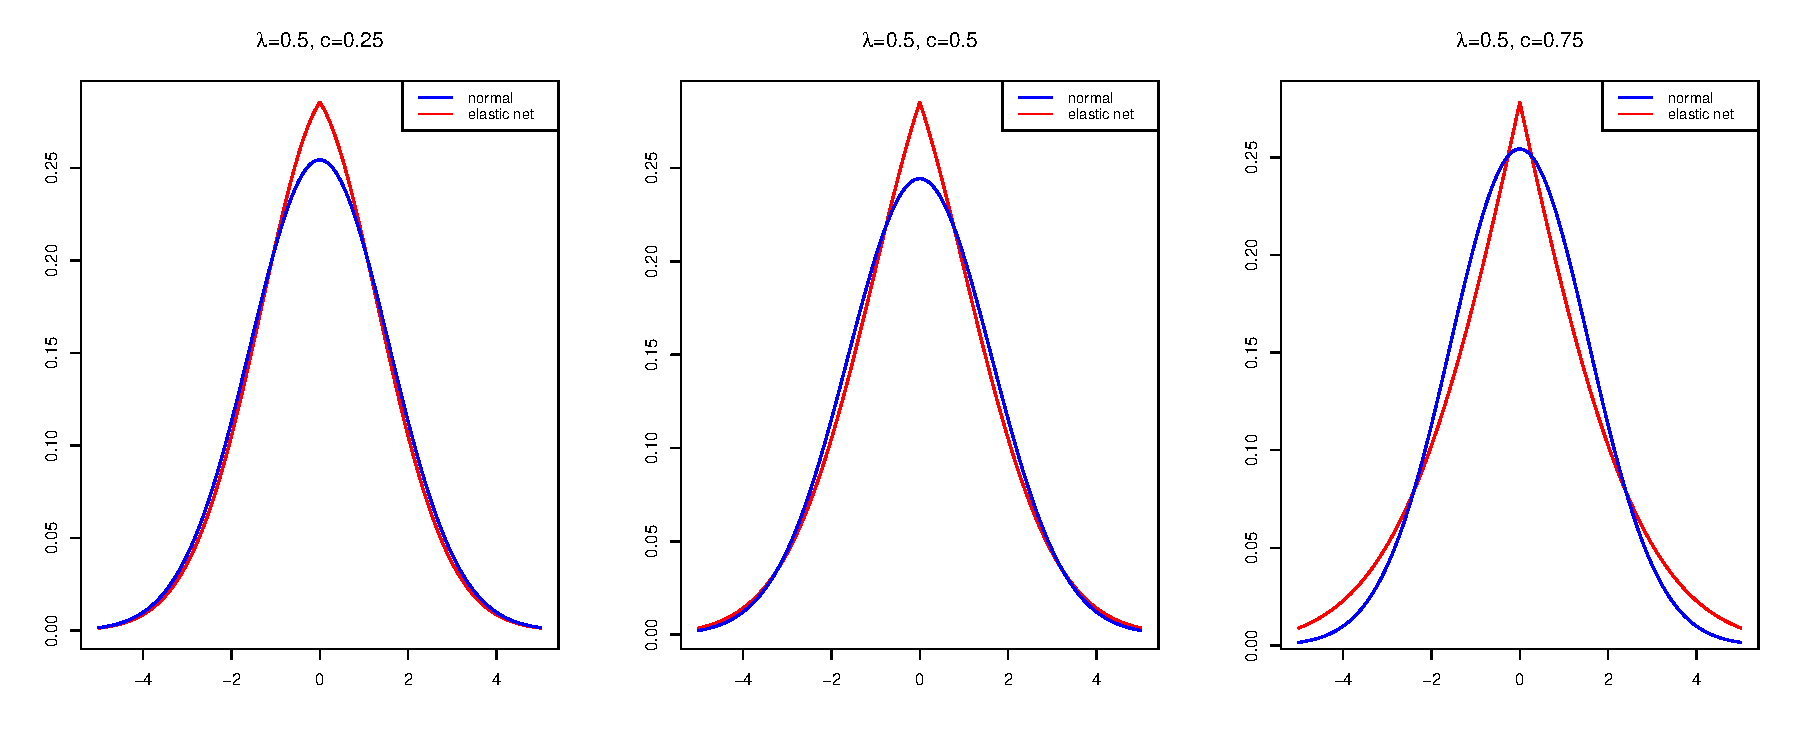
\includegraphics[width=\textwidth]{norm_appr}
  \caption{Normal approximation of the elastic net prior}
  \label{fig:norm_appr}
\end{figure}
Figure \ref{fig:norm_appr} shows the normal prior approximation compares to the elastic net prior. With the prior distribution approximation, the joint log-distribution, $\ln f(\bm{Y}, \bm{\beta};\bm{\alpha})$, then takes the form of a ridge regularized Cox regression with individual penalty parameters,
\begin{equation} \label{eq6}
\begin{aligned}
    &\ln f(\bm{Y}, \bm{\beta};\bm{\alpha}) = \sum_{l=1}^{m}\left[\sum_{i\in D_l}\bm{x}_i^T\bm{\beta}-d_l\ln(\sum_{i\in R_l} e^{\bm{x}_i^T\bm{\beta}})\right] - \sum_{j=1}^{p} \frac{1}{2}v_j\beta_j^2 + \text{const}, \\
    &v_j = \frac{2\lambda_j(1-c)+c^2\lambda_j^2}{2}.
\end{aligned}
\end{equation}
Applying the Laplace approximation \citep{laplace1986memoir} to \eqref{eq6}, the integral with respect to $p$-dimensional vector $\bm{\beta}$ has a closed form solution. Consider a Taylor series of $\ln f(\bm{Y}, \bm{\beta};\bm{\alpha})$ at the stationary point $\tilde{\bm{\beta}}$, where $\nabla \ln f(\bm{Y}, \tilde{\bm{\beta}};\bm{\alpha})=0$,
$$ \ln f(\bm{Y}, \bm{\beta};\bm{\alpha}) \approx \ln f(\bm{Y}, \tilde{\bm{\beta}};\bm{\alpha}) - \frac{1}{2}(\bm{\beta}-\tilde{\bm{\beta}})^T\bm{H}(\bm{\beta}-\tilde{\bm{\beta}}). $$
$\tilde{\bm{\beta}}$ is the solution of a ridge regularized Cox regression \eqref{eq6}, which can be computed, for fixed $\bm{\alpha}$,  using for example the  \emph{glmnet} R package \citep{simon2011regularization}. Here $\bm{H}$ is the Hessian matrix,
\begin{align*}
    \bm{H} &= - \nabla\nabla|_{\bm{\beta}} \ln f(\bm{Y}, \bm{\beta};\bm{\alpha})|_{\bm{\beta}=\tilde{\bm{\beta}}} \\
    & \approx \bm{X}^T\bm{W}\bm{X} + \bm{V}
\end{align*}
where $\bm{V} = \text{diag}[\bm{v}]=\text{diag}[v_1,\dots,v_p]$, $\bm{W}$ is a diagonal matrix with elements 
$$ \bm{W}_{ii} = \sum_{l\in C_i}\frac{d_le^{\bm{x}_i^T\bm{\beta}}}{\sum_{k\in R_l}e^{\bm{x}_k^T\bm{\beta}}} - \sum_{l\in C_i}\frac{d_l(e^{\bm{x}_i^T\bm{\beta}})^2}{(\sum_{k\in R_l}e^{\bm{x}_k^T\bm{\beta}})^2}. $$ 
The Hessian is in turn approximated to avoid computing the full matrix $W$, which is costly. Here we only use diagonal elements to speed up the computation without loss of accuracy. For greater details, refer to \cite{simon2011regularization}.
We see now that $f(\bm{Y}, \bm{\beta};\bm{\alpha})$'s Taylor approximation has a multivariate normal form with mean $\tilde{\bm{\beta}}$, and variance $\bm{H}^{-1}$. Integrating out $\bm{\beta}$ yields the normalizing constant:
\begin{equation} \label{eq7}
\begin{aligned}
    -\ln{f(\bm{Y};\bm{\alpha})} &\approx -\ln f(\bm{Y}|\tilde{\bm{\beta}};\bm{X}) - \ln \pi(\tilde{\bm{\beta}};\bm{\alpha}) - \frac{p}{2}\ln{2\pi} + \frac{1}{2}\ln{|\bm{H}|} \\
    &= -\ln{|\bm{V}|} + \tilde{\bm{\beta}}^T\bm{V}\tilde{\bm{\beta}} + \ln{|\bm{H}|} + \text{const}
\end{aligned}
\end{equation}
The approximate negative log marginal likelihood in equation \eqref{eq7} is the objective function we  minimize to estimate $\bm{\alpha}$.

\subsubsection{Marginal likelihood function optimization} \label{DCA}
Although the marginal likelihood function given by equation \eqref{eq7} is nonconvex, it can be decomposed as the difference of two convex functions: $g(\bm{\alpha}):=-\ln{|\bm{V}|} + \tilde{\bm{\beta}}^T\bm{V}\tilde{\bm{\beta}}$, and  $-h(\bm{\alpha}):=-\ln{|\bm{H}|}$. This decomposition makes it possible to use optimization algorithms specifically designed for difference of convex functions (DCA) \citep{le2015dc}. The main idea of DCA is to approximate the nonconvex objective function by a sequence of convex ones. At each iteration  we approximate the concave part ($h(\bm{\alpha}$)) by its affine majorization, i.e., the supporting hyperplane obtained by calculating its gradient, or subgradients if not differentiable, and then minimize the resulting convex approximation. The resulting algorithm can also be thought of as a majorization-minimization algorithm \citep{hunter2004tutorial}. The affine approximation of the concave part is the majorization step, which forms a surface lying above the objective function, and is tangent to it, i.e, at the current estimation of the target parameter, the majorization equals to the objective function. This ensures the majorization is a tight upper bound for the objective. Minimizing the convex upper bound is the minimization step. The DCA algorithm for the marginal likelihood $-\ln{f(\bm{Y};\bm{\alpha})}$:
\begin{enumerate}
    \item Initialize $\bm{\alpha}$ with $\tilde{\bm{\alpha}} \in \mathbb{R}^q$.
    \item Majorization: 
    \begin{itemize}
        \item calculate the gradient at current estimation $\tilde{\bm{\alpha}}$,
    $$\bm{\theta}= \nabla_{\bm{v}} \ln{|\bm{H}|} = \text{diag}[\bm{H}^{-1}]$$ 
        \item form the convex upperbound,
        \begin{align*}
        u(\bm{\alpha})&=g(\bm{\alpha})+ h(\tilde{\bm{\alpha}}) + \bm{\theta}^T(\bm{v}-\tilde{\bm{v}}) \\
        &=-\ln{|\bm{V}|} + \tilde{\bm{\beta}}^T\bm{V}\tilde{\bm{\beta}}+\bm{\theta}^T\bm{v}+\text{const}
        \end{align*}
    \end{itemize}
    \item Minimization: $\hat{\bm{\alpha}}=\underset{\bm{\alpha}}{\operatorname{\argmin}} \left\{u(\bm{\alpha})\right\}$.
    \item Set $\tilde{\bm{\alpha}} = \hat{\bm{\alpha}}$.
    \item Repeat step 2-4 until convergence of $\hat{\bm{\alpha}}$.
\end{enumerate}
The minimization of $u(\bm{\alpha})$ can be performed with a standard first order method like gradient descent, or a second order method like Newton-Raphson. The gradient and Hessian of $u(\bm{\alpha})$ are:
\begin{align*}
    &\nabla_{\bm{\alpha}} u(\bm{\alpha}) = \bm{Z}^T\left[(-\frac{1}{\bm{v}}+\tilde{\bm{\beta}}^2+\bm{\theta})((1-c)\bm{\lambda}+c^2\bm{\lambda}^2)\right],\\
    &\nabla\nabla_{\bm{\alpha}} u(\bm{\alpha}) = \bm{Z}^T \text{diag}\left[\frac{\bm{\lambda}^2}{\bm{v}^2}(1-c+c^2\bm{\lambda})^2+(-\frac{1}{\bm{v}}+\tilde{\bm{\beta}}^2+\bm{\theta})\bm{\lambda}(1-c+2c^2\bm{\lambda})\right]\bm{Z}.
\end{align*}

\subsection{Summary} \label{cha3_sum}
We incorporate the meta-features into feature-specific penalty parameters modeled as a log-linear functions of the meta-features. We then use a Bayesian interpretation of regularized regression to obtain the marginal likelihood function for the meta-feature weights $\bm{\alpha}$. The $\bm{\alpha}$ parameter are estimated by maximum marginal likelihood. The resulting nonconvex objective function can be decomposed into a difference of two convex functions, which can be optimized with a difference of convex functions algorithm. The estimated $\bm{\alpha}$ can be plugged in  to compute the penalty parameters. The complete model fitting procedure is given by:
\begin{enumerate}
    \item Initialize $\bm{\alpha}$ with $\tilde{\bm{\alpha}}$.
    \item Repeat, until convergence of $\hat{\bm{\alpha}}$.
    \begin{enumerate}
        \item Laplace approximation of marginal likelihood with known $\tilde{\bm{\alpha}}$, section \ref{laplace},
        \begin{itemize}
            \item Approximate the elastic net prior with a normal prior, equation \eqref{eq6},
            \item Calculate $\tilde{\bm{\beta}}$ and $\bm{H}$.
        \end{itemize}
        \item Optimize Laplace approximation of marginal likelihood, equation \eqref{eq7}, get solution $\hat{\bm{\alpha}}$, with DCA described in section \ref{DCA}.
        \item Set $\tilde{\bm{\alpha}} = \hat{\bm{\alpha}}$.
    \end{enumerate}
    \item Calculate customized penalty vector $\bm{\lambda}=e^{\bm{Z}\hat{\bm{\alpha}}}$.
    \item Fit regularized Cox regression, equation \eqref{eq2}, with $\bm{\lambda}$.
\end{enumerate}

\subsection{Inclusion of unpenalized features}
We have introduced the computational algorithm for meta-feature guided regularized regression \eqref{eq2}, in which all the features are regularized, and have meta-features associated with them. However, more often than not, there are other types of features providing substantial predictive power to the outcome, in addition to genomics. For example, demographics like age at diagnosis, gender; clinical features such as symptoms, imaging and lab results. These features usually do not have meta-feature information and it is desirable to include them in the model without penalization. To extend our model to include unpenalized features, we denote unpenalized feature matrix $\bm{X}'_{n\times p'}$, i.e., there are $p'$ unpenalized features; $\bm{\beta}'\in \mathbb{R}^{p'}$ is the coefficient vector for them. Then \eqref{eq2} can be rewritten as
\begin{equation} \label{eq8}
\begin{aligned}
    &\min_{\bm{\beta}'\in \mathbb{R}^{p'}, \bm{\beta}\in \mathbb{R}^p} \left\{-\ell(\bm{\beta}', \bm{\beta}) + \sum_{j=1}^p \lambda_j\left[\frac{1}{2}(1-c)\beta_j^2 + c|\beta_j|\right]\right\}, \\
    &\lambda_j = e^{\bm{z_j}^T \bm{\alpha}}.
\end{aligned}
\end{equation}
The only difference between \eqref{eq8} and \eqref{eq2} is the addition of unpenalized features $\bm{X}'$ and their coefficients $\bm{\beta}'$ in log partial likelihood $\ell(\bm{\beta}', \bm{\beta})$. If we walk through the algorithm described in section \ref{cha3_sum}, the procedures will follow. Except that the alternating optimization of $\bm{\beta}$, $\bm{\alpha}$ now takes place with $(\bm{\beta}', \bm{\beta})$, $\bm{\alpha}$, and $\bm{\beta}'$ is estimated using regularized regression with their $\lambda$ being 0.

\section{Simulations}
\subsection{Simulation methods}
In this section, we perform a series of simulation experiments to evaluate the performance of the proposed model in terms of prediction and feature selection performance compared to standard regularized Cox regression. We first generate meta-feature data $\bm{Z}$ by sampling from independent Bernoulli variables, with probability 0.1. This is to mimic biological pathway/functional gene set meta-features. Each pathway contains a group of genes, and 1 indicates the gene belongs to the pathway and 0 if the gene does not. Meta-feature weights $\bm{\alpha}$ were fixed from an equally spaced grid of values ranging from -1 to 1. We then generate $\bm{\beta}$ from a normal prior distribution with mean 0, and variance computed from $\bm{\alpha, Z}$, based on equation \eqref{eq5}. Because we want the underlying model to be sparse, we only keep the top 20\% of the $\bm{\beta}$ elements with largest absolute values, and set the remaining to be 0. To model uninformative meta-features we also consider scenarios where we randomly flip some of the rows of $\bm{Z}$ from 0 to 1 or vice versa. The proportion of modified rows, tracks the overall informativeness of meta-features, e.g., 10\% of the rows modified corresponds to high informativeness while 90\% of the rows modified corresponds to low informativeness. The rows of the data matrix $\bm{X}$ are sampled from a multivariate normal distribution with autoregressive correlation structure, $\bm{\Sigma}_{ij} = \rho^{|i-j|}$, with $\rho=0.5$. Survival times are generated using the inverse probability integral transform:   
\begin{displaymath}
t = H_0^{-1}\left(-\ln(U)e^{-\bm{\beta}^T\bm{x}}\right)
\end{displaymath}
where $U\sim \text{uniform}[0,1]$, $H_0(t) = (t/5)^8$ is a baseline cumulative hazard function with Weibull distribution. Censoring times are sampled from an exponential distribution, $c\sim \text{exp}(0.1)$. The parameter values for the Weibull and exponential distributions are set to generate survival times in the 0 to 20 range, and a fixed ratio (3/2) of events to censoring. We then add normal noise to survival times to control the overall underlying predictive ability of the features for the outcome. Specifically, we set the concordance measure \citep{harrell1982evaluating} to 0.8, by controlling the standard deviation of the added noise. The survival outcome is set to be the minimum of the generated survival and censoring time, $y=\text{min}(t,c)$.

For each simulation replicate, we generated training data as described above. We then fit a standard elastic net regularized Cox regression without external meta-features $\bm{Z}$, and also fit our proposed model with meta-features. Elastic net regression is tuned with 5-fold cross validation, while the proposed model does not require penalty parameter tuning as it is estimated as part of the model fitting procedure. We then compare the prediction performance between the two models on an independent test set of size 1000 generated following the same procedure described for the training data. We used the C-index as a performance metric. For each simulation scenario we used 100 replicates. 

We run a series of experiments varying one key parameter while keeping the others fixed. The base case parameters are sample size $n=100$, feature size $p=200$, meta-feature size $q=10$, meta-feature $\bm{Z}$ informativeness: 5\% of features (rows of $\bm{Z}$) modified to have incorrect values. Four experiments are conducted by varying one parameter at a time.
\begin{enumerate}
    \item Meta-feature informativeness level from high to low, proportion of rows of $\bm{Z}$ modified 5\%, 15\%, 30\%.
    \item Feature size, $p=200, 600, 1000$.
    \item Sample size, $n=100, 200, 300$.
    \item Meta-feature size, $q=10, 20, 30$.
\end{enumerate}
In experiment 1, we also examined the feature selection performance by both models, to evaluate how informativeness of meta-features influences model interpretation.

\subsection{Simulation results}
Figure \ref{fig:sim21} shows the results of the 4 simulation experiments. The horizontal dashed line in each panel represents the population/theoretical C-index, achievable with infinite samples of training data. It is provided as a reference for each parameter setting. The performance of the meta-feature guided elastic net Cox model (denoted as `meta' in the figure) is compared to that of a standard elastic net Cox model. 

In experiment 1, there are consistent improvements in prediction performance as long as the meta-features are informative. The higher the informativeness of meta-features, the larger the gains in prediction performance over the standard elastic net model.

Experiment 2 illustrates the model performance with respect to the number of features $p$. Larger number of features relative to the sample size makes it harder for both models to predict well, as both models' test C-index are substantially below the theoretical C-index of 0.8, when $p=600$ or $p=1,000$. However, the meta-feature model consistently outperforms the standard elastic net model.

Experiment 3 evaluates a similar situation as experiment 2, but instead of varying the number of features, it varies the sample size $n$ while keeping $p=200$. As the sample size gets larger, i.e, the ratio of number of features to sample size  becomes smaller, both models perform better, and the meta-feature guided elastic net consistently outperforms the standard elastic net. Furthermore, a larger sample size yields more stable prediction metrics (smaller variance of test C-index). 

As the size of meta-features increases (experiment 4), the prediction performance improvement over the standard elastic net becomes smaller. This indicates the meta-feature guided model's inability to handle a large number of meta-features.  

In terms feature selection performance, we define accurate selection as follow: features with non-zero simulated coefficients are estimated with non-zero values and features with zero simulated coefficients are estimated as zero. In Figure \ref{fig:sim22}, we compared the feature selection accuracy of the meta-feature guided elastic net model, standard elastic net model with the $\lambda$ value that gives maximum cross-validated C-index (denoted as `enet.min'), and with the $\lambda$ value that gives the most regularized model such that the cross-validated C-index is within one standard error of the maximum (denoted as `enet.1se'), in experiment 1, where the informativeness of meta-features varies. The `1se' elastic net model is sparser (fewer nonzero coefficients) than the `min' elastic net model. The proposed meta-feature guided elastic model again outperforms both standard elastic net models in feature selection accuracy. Moreover, the selection is more stable with meta-features compared to either of the standard elastic net models. Note that the selection accuracy of the `min' elastic net model is highly unstable, since it yields less sparse models than the `1se' elastic net, and the meta-feature guided model.
\begin{figure}
    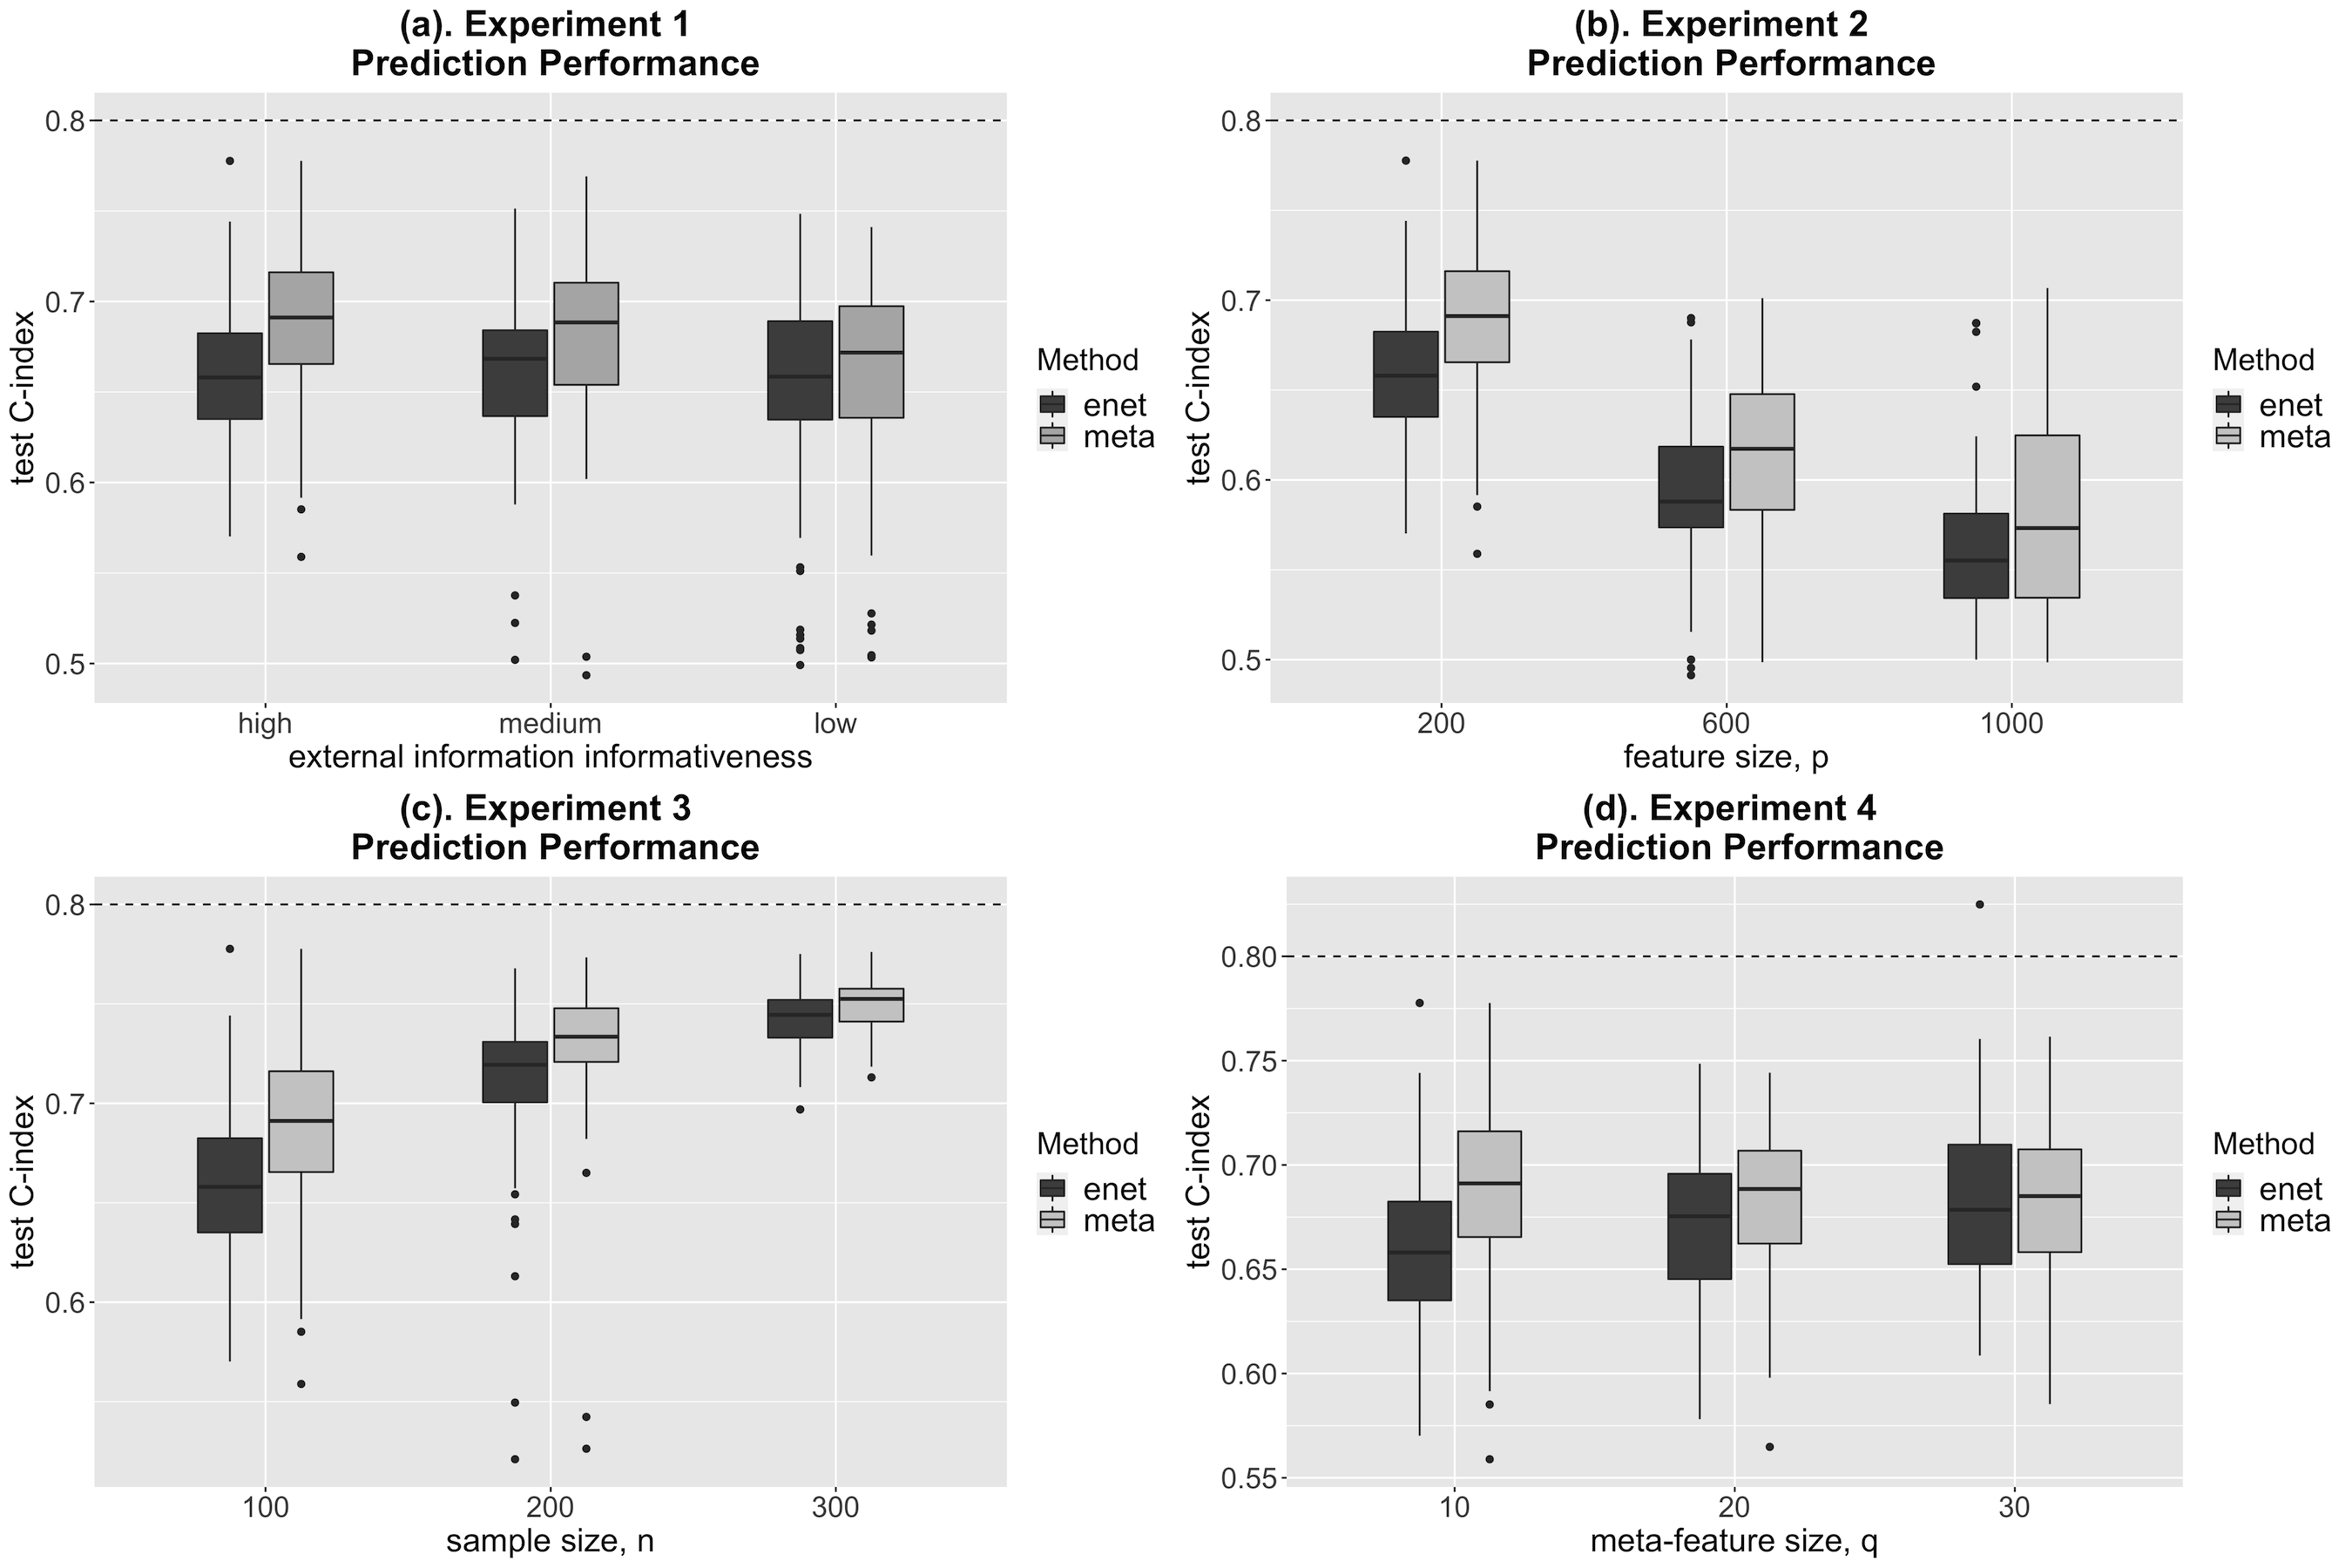
\includegraphics[width=\textwidth]{sim21}
    \caption[Simulation results (meta guided): prediction performance] {Simulation result: prediction performance}
    \label{fig:sim21}
\end{figure} 

\begin{figure}
    \centering
    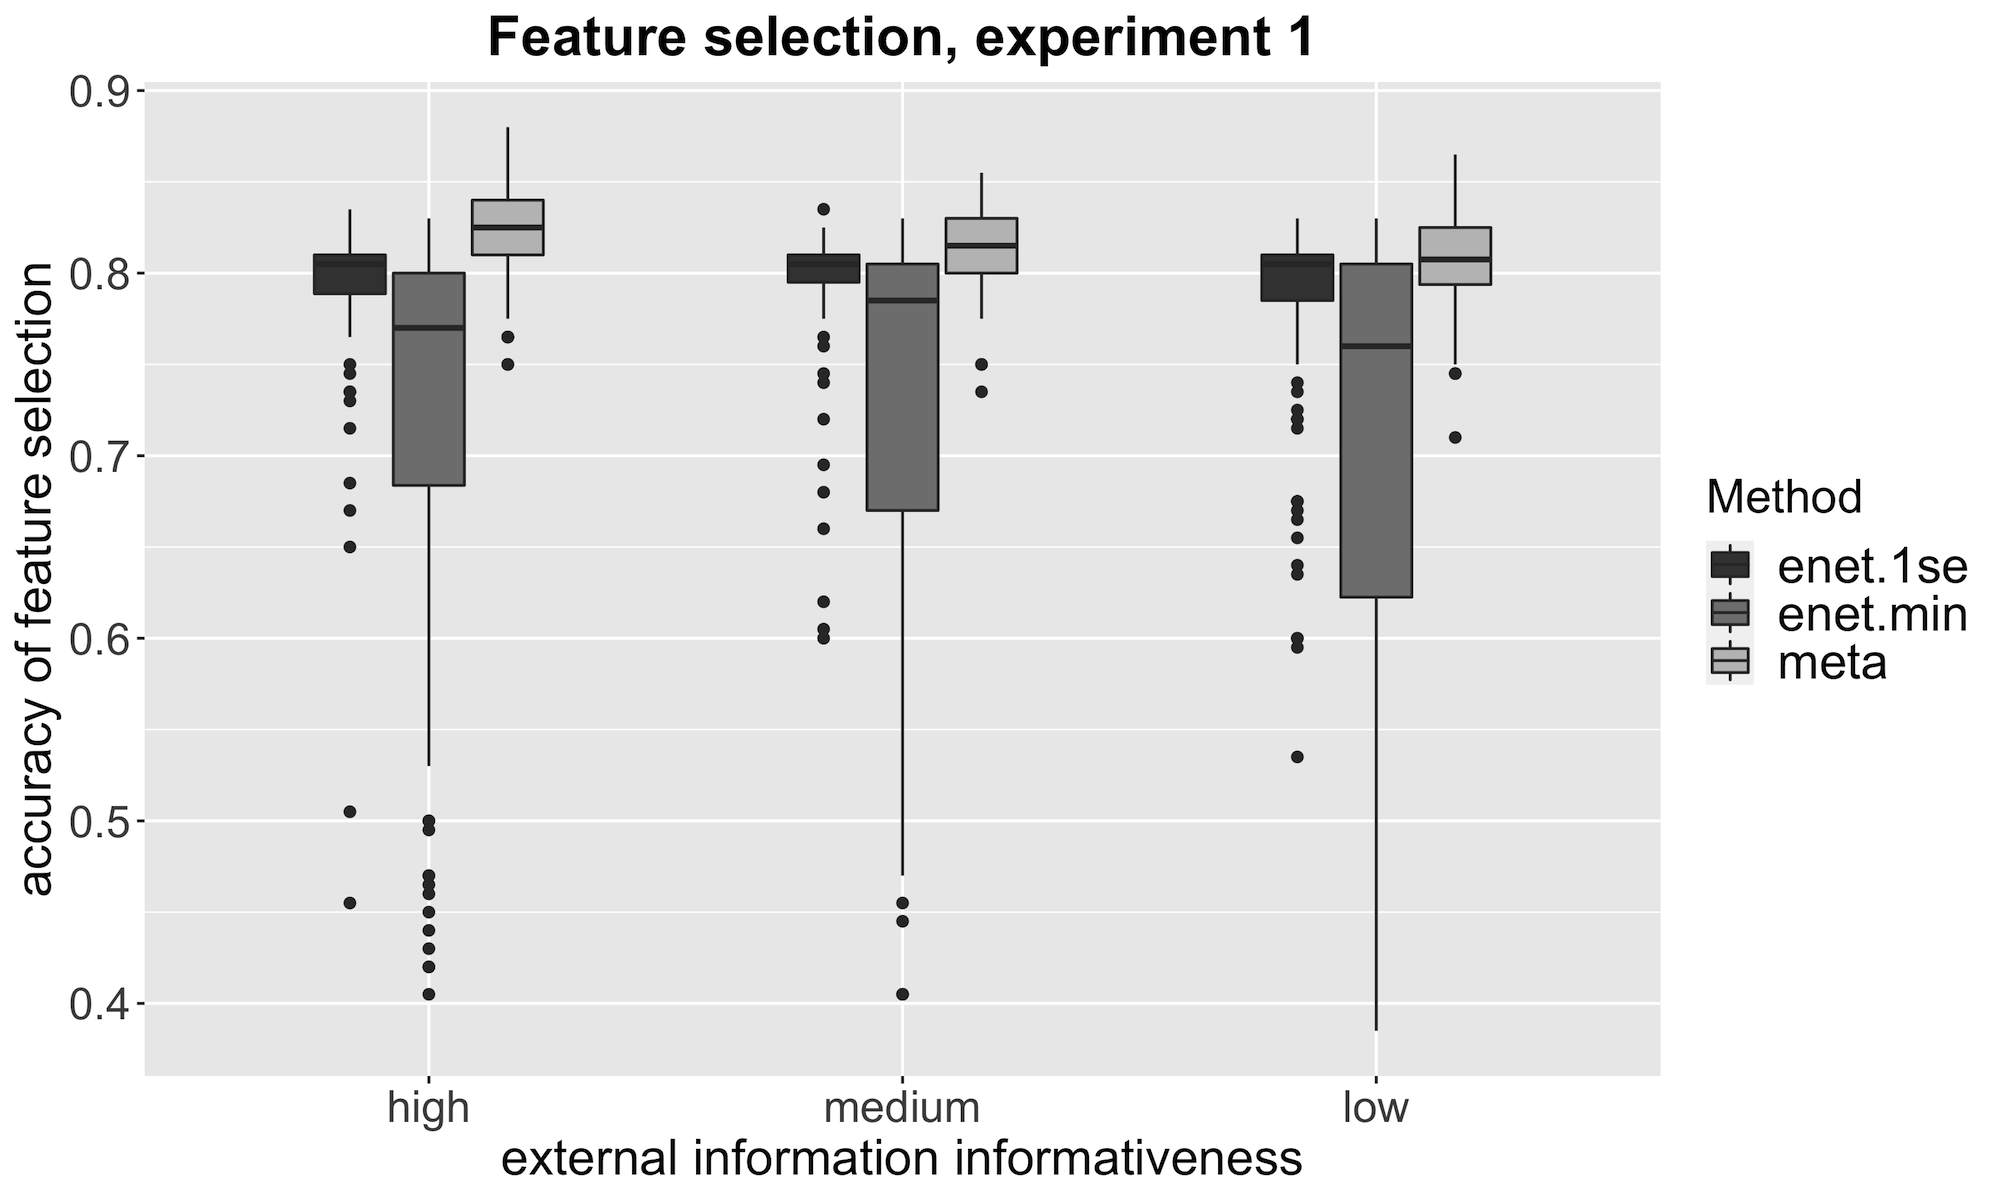
\includegraphics[scale=0.7]{sim22}
    \caption[Simulation results (meta guided): feature selection]{Simulation results: feature selection. `enet.min' is the standard elastic net model with the $\lambda$ value that gives maximum cross-validated C-index; `enet.1se' is the elastic net model with the $\lambda$ value that gives the most regularized model such that the cross-validated C-index is within one standard error of the maximum.}
    \label{fig:sim22}
\end{figure}

\section{Applications}
\subsection{Gene expression signatures for breast cancer survival}
To illustrate the performance of our approach in real data, we applied the meta-feature guided regularized regression to the Molecular Taxonomy of Breast Cancer International Consortium (METABRIC) study. The data includes cDNA microarray profiling for close to 2,000 breast cancer specimens processed on the Illumina HT-12 v3 platform (Illumina\_Human\_WG-v3) \citep{curtis2012genomic}. The data was divided into a discovery/training set of 997 samples, and a validation/test set of 995 samples. The goal is to build a prognostic model for breast cancer survival, based on gene expressions and clinical features. The feature data $\bm{X}$ consists of of 29,477 gene expression probes and two clinical features, age at diagnosis and the number of positive lymph nodes. The meta-feature data $\bm{Z}$ consists of four ``attractor metagenes'', which are selected gene co-expression signatures  associated with the ability of cancer cells to divide uncontrollably, to invade surrounding tissues, and, with the effort of the organism to fight cancer with a particular immune response \citep{cheng2013biomolecular}. Three metagenes are universal “attractor metagenes” and consist of  genes involved in mitotic chromosomal instability (CIN), in mesenchymal transition (MES), and lymphocyte-specific immune recruitment (LYM) respectively. A fourth metagene is associated with good prognosis and contains two genes: FGD3 and SUSD3. The CIN, MES, and LYM metagenes each consist of 100 genes, but for our analysis, we considered only the 50 top-ranked within each metagene. The data matrix $\bm{Z}$ is an indicator matrix for whether a specific expression probe corresponds to a gene in a metagene. 

Model building was based on the samples with ER positive and HER2 negative, as treatments are more homogeneous in this group, and they are associated with good prognosis \citep{rivenbark2013molecular}. There were 740 samples in the discovery set and 658 samples in the validation set in the ER+ and HER2- subset after removing samples with missing values. We applied meta-feature guided elastic net regression to train the model. The test set was used to evaluate model performance. The same training/test scheme was used to fit a standard elastic net regression without attractor metagene information as comparison. 

With only gene expression features in the model and no clinical features, the test C-index for the metagene guided elastic net model is 0.637 compared to the test C-index of 0.663 for the standard Cox elastic net counterpart. When adding the clinical features, age at diagnosis and number of positive lymph nodes, the test C-index increased to 0.715, and 0.728 for the metagene guided elastic net model, and the standard Cox elastic net model, respectively (Table \ref{table1}). Our metagene guided elastic net model does not perform as well as the standard elastic net model, in both situations, with or without clinical features. This contrasts with the experience with `xrnet', which improved performance in the METABRIC data. To understand the difference, we looked at the metagene weights estimated from the empirical Bayes method. Intercept represents the penalty applied to probes that do not map to any of the metagenes. The metagene weights indicates the differential penalty amount applied to the genes in the metagene; a positive (negative) weight will have the genes in the metagene penalized more (less) strongly, indicating they are less (more) important for predicting the mortality. The metagenes `CIN' and `FGD3-SUSD3' are more important than `MES' and`LYM', conforming to the findings with `xrnet' (chapter \ref{cha:xrnetcox}, section \ref{app:meta2}). Also, the number of features selected by metagene guided model is much less than that of standard elastic net, 9 vs 30 for gene expression only, and 9 vs 49 for gene expression plus clinical features, respectively. These findings suggests that although the methods agree in identifying which  metagenes are more important, non-linear integration of meta-features does not fit well the specific data and that the underlying relationship between gene expressions and metagenes in METABRIC is better captured by the linear model implicit in `xrnet'.  
\begin{table}[tbh]
    \centering
    \def\arraystretch{1.5}
    \begin{tabular}{|c|c|c|c|}
        \hline
        \multicolumn{2}{|c|}{} & \textbf{Elastic net} & \textbf{Metagene elastic net} \\ 
        \specialrule{.1em}{.05em}{.05em}
        \multirow{2}{*}{\textbf{C-index}} & Gene expressions only & 0.663 & 0.637 \\ 
        & Gene expressions + clinical & 0.728 & 0.715 \\ 
        \hline
    \end{tabular}
    \caption{METABRIC: Test C-index between standard elastic net and metagene guided elastic net}
    \label{table21}
\end{table}

\begin{table}[tbh]
    \centering
    \def\arraystretch{1.5}
    \begin{tabular}{|c|c c|}
        \hline
        \multirow{2}{*}{\textbf{Metagene}} & \multicolumn{2}{ c|}{\textbf{Metagene weights $\alpha$}} \\
         & Gene expressions only & Gene expressions + clinical \\
        \specialrule{.1em}{.05em}{.05em}
        Intercept & 4.7355 & 4.7582 \\
        \hline
        CIN & -1.3677 & -1.4057 \\
        \hline
        MES & 0.5520 & 0.7581 \\
        \hline
        LYM & 0.1074 & 0.2953 \\
        \hline
        FGD3-SUSD3 & -2.0187 & -1.8620 \\
        \hline
    \end{tabular}
    \caption{METABRIC: Metagene weights $\alpha$}
    \label{table22}
\end{table}

\subsection{Anti-PD1 predictive biomarker for melanoma survival}
We also applied the proposed meta-feature model to a melanoma data set to predict overall survival in patients treated with PD-1 immune checkpoint blockade. The programmed death 1 pathway (PD-1) is an immune-regulatory mechanism used by cancer to hide from the immune system. Antagonistic antibodies to PD-1 pathway and its ligands, programmed death ligand 1 (PD-L1), demonstrate  clinical benefits and tolerability. Immune checkpoint blockades such as Nivolumab, pembrolizumab are anti-PD-1 antibodies showing improved overall survival for the treatment of advanced melanoma. However, less than 40\% of the patients respond to them \citep{moreno2015anti}. Therefore,  identifying predictive signals of treatment outcomes is of great interest to select patients most likely to benefit from anti-PD-1 treatment. We explored transcriptomes and clinical data using our model to illustrate prediction performance and predictive signal selection.

The dataset combined 3 clinical studies in which RNA-sequencing profiles of patients treated with anti-PD1 antibodies was obtained: \cite{gide2019distinct, riaz2017tumor, hugo2016genomic}. The gene expression levels were normalized toward all sample average in each study as the control, so that they are comparable to one another across features within a sample and comparable to one another across samples. There are 16,010 genes in common across the 3 studies, and a combined total of 117 subjects. The clinical variables being considered are age, gender, and tumor response. We build predictive models for overall survival based on transcriptomics and clinical variables. Since the subjects are all treated with anti-PD1 antibodies, the transcriptomic features selected by the model are predictive signals for treatment efficacy or resistance. We selected hallmark gene sets as meta-features from the molecular signature database  \citep{liberzon2015molecular}. A total of 13 gene sets were enriched \citep{subramanian2005gene} with false positive rates less than 0.25 (Table \ref{table3.1}). The meta-feature matrix is formed as an indicator of whether each of the 16,010 genes belong to one of the 13 hallmark gene sets ($\bm{Z}$). 

We compared prediction and feature selection performance between the meta-feature guided elastic net model and the standard elastic net model. The data is split into training ($75\%$) and test set ($25\%$). Standard elastic net was trained using 5-fold cross validation, while the meta-feature model was trained with estimated hyperparameters. The test concordance index is C = 0.7340 for the elastic net, and C = 0.7609 for our meta-feature guided model. As for feature selection, the meta-feature model, which selects 4 genes (GPAA1, COX6C, VPS28, PLCB4), is sparser, compared to 11 genes selected in the elastic net model. 
\begin{table}[tbh]
    \centering
    \def\arraystretch{1.3}
    \begin{tabular}{|c|c|}
    \hline
     \bf Hallmark meta-feature & \bf Estimated $\bm{\alpha}$ \\
     \specialrule{.1em}{.05em}{.05em}
     Interferon gamma response & -0.0102  \\ \hline
     Allograft rejection & 0.1570  \\ \hline
     Interferon alpha response & -0.0314 \\ \hline
     IL6 JAK STAT3 signaling & 0.1131 \\ \hline
     Inflammatory response & 0.0744 \\ \hline
     Complement & 0.1577 \\ \hline
     TNFA signaling via NFKB & 0.1180 \\ \hline
     IL2 STAT5 signaling & 0.1613 \\ \hline
     Bile acid metabolism & 0.0876 \\ \hline
     Kras signaling down & 0.2338 \\ \hline
     Xenobiotic metabolism & 0.2598 \\ \hline
     Apoptosis & 0.2557 \\ \hline
     Kras signaling up & 0.2737 \\ \hline
    \end{tabular}
    \caption[Anti-PD1: List of hallmark meta-features and their respective estimated weight]{Anti-PD1: List of hallmark meta-features and their respective estimated weight $\bm{\alpha}$.}
    \label{table3.1}
\end{table}

\section{Discussion}
In this chapter, we extended to survival outcomes the customized regularization model guided by genomic meta-features of \cite{zeng2021incorporating}. This model has individualized penalty parameters for each of the features instead of the single global penalty parameter traditional in commonly used regularized regression methods. Differential penalization allows for the importance of each feature in predicting the outcome of interest to be determined from the data by their underlying characteristics/meta-features. With  informative meta-features, the more important features will be penalized less, resulting in a lower  likelihood of being shrunk to exactly 0, and for the less important features to be more strongly penalized, resulting in a higher likelihood of being excluded from the model. In our simulation experiments and the anti-PD1 immunotherapy predictive modeling application, the customized regularization model showed benefits in prediction performance, and the selected model tended to be sparser (fewer features selected). Of note is that to derive prediction performance gains, the external meta-feature data needs to be  informative and low-dimensional. Therefore,   substantive pior knowledge to carefully select a potentially relevant and limited meta-features set is critical. 

We have developed two different methods to systematically integrate meta-feature information into the modeling process with survival outcomes and high-dimensional data. The approach in this chapter integrates meta-features in a non-linear way. It allows the meta-features to dictate the importance of each feature by defining the penalty parameters as a non-linear function of the meta-features. By contrast, the `xrnet' regularized hierarchical model in chapter \ref{cha:xrnetcox} integrates meta-features linearly. The fundamental difference between the two methods is that `xrnet' models meta-features through the mean of $\bm{\beta}$, while the proposed model in this chapter models meta-features through the variance of $\bm{\beta}$. Specifically, `xrnet' models $\bm{\beta} \sim N(\bm{Z\alpha}, \tau\bm{I})$, and the customized regularization approcah models $\bm{\beta}$ as having an approximate prior $N(0, \frac{2}{2\lambda_j(1-c)+c^2\lambda_j^2})$. In most scenarios, a user would not know which model to favor in advance. Depending on the application at hand, one would want to consider both approaches, selecting the best based on the performance on test data. 

Our proposed model applied empirical Bayes to estimate penalty parameters for each feature, which uses the Laplace approximation to obtain the marginal likelihood. However, the Laplace approximation works well when sample size is relatively large. We see in simulation experiment 2, that while our model shows prediction benefits in all feature set sizes, there is a decreasing gain trend over standard elastic net Cox regression, which maybe caused by the drop in the quality of the Laplace approximation when the sample size is  small relative to the feature set size.  But we did not directly assessed how well the Laplace approximation affects the model performance. 

We have already mentioned that the proposed customized regularization model does not handle well high-dimensional  meta-features. This is because no regularization is applied to the meta-feature weights $\bm{\alpha}$, or other mechanism to control the complexity of this part of the model. As a result, the model fitting algorithm is not able to deal with large number of meta-features efficiently and stably. Careful filtering of the meta-features is then required in a high-dimensional meta-feature setting. Future work to regularize the meta-feature part of the model is a potential improvement to expand its ability of handling high dimensional meta-feature data.
